\documentclass[12pt,a4paper]{article}
\usepackage[utf8]{inputenc}
\usepackage{amsmath}
\usepackage{blkarray}
\usepackage{amsfonts}
\usepackage{amssymb}
\usepackage{makeidx}
\usepackage{graphicx}
\usepackage{lmodern}
\usepackage{url}
\usepackage{color}
\usepackage[dvipsnames]{xcolor}
\usepackage{bm}
\usepackage{booktabs}
\usepackage{float}
\usepackage{listings}
\usepackage[left=2cm,right=2cm,top=2cm,bottom=2cm]{geometry}
\author{Mudathir Mahgoub \\ 0119655301}
\title{Takehome Midterm Exam 2}
\begin{document}

\maketitle


\begin{enumerate}

\item Explain the differences between cross-site scripting (XSS) and cross-site
request forgery (CSRF) attacks in your own words. Describe a fictitious scenario in
which CSRF can be used to leak confidential information about the victim user. Finally,
explain the confused deputy problem in your own words. Give an example of a web
attack that occurs as the browser acts as the confused deputy.

\color{blue}
XSS enables an adversary to inject malicious script into the dom of a website that is passed to the client. 
That script can hijack the browser cookies including authentication tokens which may be sent to the adversary. CSRF on the other hand doesn't steal browser cookies, but tricks the browser into sending new  requests to different websites (like facebook) using the authentication cookies for that website. If the user is already authenticated, the browser can't distinguish this forged request from a valid one and would supply the required cookies with the request. If the victim website is vulnerable, the request would be accepted as a valid one and the request would be served. For example if the forged request is changing the password and the server accepts that request, then the adversary has succeeded in gaining access to the victim account. 

Confused deputy problem is when a program with higher permissions is tricked to perform actions that require higher permission for users with lower permissions. CSRF is an example where the browser is the confused deputy. The browser keeps track of authentication cookies for websites where the user is logged in, and supplies these cookies when the user accesses these websites. The CSRF attack exploits this feature by tricking the browser to send these cookies in forged requests (e.g. links or Ajax request) and the browser can't distinguish these forged requests from real ones. 
\color{black}

\item Explain the ``Spectre attack" in your own words and identify the goal of
the adversary for this attack. What is the fundamental weakness of the system that
the attackers exploit in the Spectre attack? What is the impact of the Spectre attack?
In your own words, give a scenario in which an attacker can exploit Spectre attack to
achieve something malicious.


\color{blue}
Spectre attack exploits the speculative execution feature available in modern processors which is used to enhance the performance. Instead of idly waiting for values in memory to be loaded inside the CPU before executing a path, speculative execution predicts a path of execution and attempts to execute that path in advance before the values that determine the actual path are retrieved from memory. If the prediction is correct, no need to execute the path  because it is already executed and only the result need to be committed. If the prediction is wrong, the CPU reverts back to the state before the prediction and continues execution from there with performance compared to being idle. When the vulnerable CPU speculatively executes the predicted path, it can access locations in isolated memory like the memory of other processes and bring their values into the caches and CPU registers. The adversary exploits this vulnerability by training the CPU to predict a certain branch using legitimate memory locations within his memory space. When the CPU learns the predicted path, then adversary changes the memory locations to point to addresses outside his address space and the CPU will retrieve these memory locations into the cache and its registers. When the CPU detects that the execution path is incorrect, it reverts its registers and state, but the memory values of the other processes in the cache remain unchanged which can be accessed by the adversary. By repeating Spectre attack, the adversary can read all memory values of other processes. However, the adversary can't write values into memory addresses outside his address space.

Any processor with speculative execution is prone to Spectre attack, therefore most modern processors of desktops, servers, and mobile devices are susceptible to Spectre attack including processors from vendors like Intel, AMD and ARM. It is difficult to defend against Spectre attack because the vulnerability is in the CPU which is difficult to change. So the feasible approach is to change the design of new processors. 

Spectre attack enables adversaries to  read to confidential contents stored in memory and registers. However the contents integrity are preserved. Once scenario is when there are multiple virtual machines running in a physical server in the cloud. Typically the adversary has access only to his virtual machine. However with Spectre attack adversary can read the memory of other virtual machines running on the same server, and obtain secret information like secret keys secret messages. 
\color{black}

\item How does the different cryptographic currency schemes (e.g., Bitcoin) ensure
that an arbitrary adversary cannot bundle up some arbitrary transactions to make a
block and add it to the blockchain? Explain the process in your own words. Why is it
the case that an attacker can double spend only if he possesses 51\% of the computing
power of the whole network? Explain how is it possible.


\color{blue}

In cryptocurrency, a typical user would have one or more addresses (similar to bank accounts). These addresses are public keys for elliptic curve digital signature algorithm. When the user makes a transaction, he signs the transaction using his private key so that others can verify the signature using his public address. Normally the transaction would be sent to a bookkeeper to be added to the global block chain. 
A transaction is considered posted when it is added to a block that is appended to the block chain by a bookkeeper (similar to posting to the general ledger). A transaction contains the key information \textbf{From Addresses} (similar to from accounts), \textbf{To Addresses} (similar to to accounts),  and \textbf{Amount} besides other information like the fee of the bookkeeping. The bookkeeper verifies the transaction and its signature, and checks the balances are valid using the information in the global block chain. If the transaction is valid, the bookkeeper will add it along with other transactions in one block. Then it solves a hashing puzzle that requires 10 minutes computation and stores the solution in the block before appending it to the black chain and broadcasting it to other bookkeepers. Now the block chain is updated and other bookkeepers would use it in later transactions.


Any user can act as a bookkeeper for the block chain (which is around 149 gigabytes in 2017 \footnote{\url{https://www.statista.com/statistics/647523/worldwide-bitcoin-blockchain-size/}}). So an adversary can act as a bookkeeper as well. Actually I think an adversary can create arbitrary transactions by sending money from \textbf{his addresses} to other addresses given that he has enough balance of bitcoins. But of course this is useless to the adversary and he will loose electricity for computation and doesn't gain any thing. However the adversary can't send money from addresses he doesn't own because transactions need signatures using the private keys of these addresses which are unknown to the adversary. Therefore other bookkeepers in the bitcoins network would reject the added block simply because the signatures verification would fail.  

Double spending is when a user attempts to post 2 transactions (or more) with balance not enough for all transactions altogether, but enough for each transaction separately. Posting these transactions one after another wouldn't work because the second transaction would be rejected by the bookkeeper due to no enough balance. If the user attempts to post the 2 transaction simultaneously to the same bookkeeper, it would reject them because the balance is not enough for the 2 transactions. So the only choice left for the user is to send each transaction to a different bookkeeper at the same time. Now it is possible both bookkeepers accept the transactions and update the block chain and end up with 2 versions for the block chain. When the 2 bookkeepers broadcast the block chains, the bookkeepers in the network would vote to choose only one of them. The block chain with the majority votes wins and bookkeepers would use it to add more blocks. Typically bookkeepers choose the longest chain and discard the others.  Therefore service providers need to wait until the longest chain is synchronized across bookkeepers before providing the requested service to the user. The waiting time normally is one hour or 6 blocks after the one with the posted transaction. 

For an adversary to double spend, he needs to post the first transaction and wait for one hour (6 blocks) for it to be approved by the service provider. At the same time, he needs to work on the branch of the second transaction privately and add more blocks at a rate faster than other bookkeepers in the network. After one hour the adversary would have a longer black chain that he can release and be selected by other bookkeepers which means the success of the double spending.

However the adversary needs computation power to solve the hashing puzzles faster than other bookkeepers in order to have a longer block chain. The computation power needed is 51\% of the computing power of the whole network.  



\color{black}

\item Explain the buffer overflow attack. Your description of the attack should
include the weakness of the system that the adversary exploits, the objective of the
adversary in this attack, and the steps the adversary should take to carry out this
attack. Describe the different defenses (e.g., Canary, ASLR) that can thwart the buffer overflow attack, and discuss their relative advantages and disadvantages. Can you have buffer overflow attacks in a program written in Java? Please explain your answer.


\color{blue}
Buffer overflow attack is writing more data into a buffer in a way that exceeds its boundaries to cause the running software to crash or behave unexpectedly. The objective of the attacker can just be the crash itself, or  the execution to jump to an address that contains malicious code. 

Canary token or a security token is a random number that is generated and stored in the stack before a function is called and should not change when the function returns. If the token is changed after the function returns, then memory corruption is detected and perhaps caused by buffer overflow. The program can then log the event and exit. Canary tokens enable detecting buffer overflow, but decrease the performance because of the security tokens management overhead.

Address Space Layout Randomization is another way to defend against buffer overflow attacks which rely on fixed addresses in the stack and the heap of a program, or fixed addresses of shared libraries. ASLR avoids this by randomizing the addresses of the heap, stack and shared libraries. This address randomization makes it difficult for injected code by buffer overflow attack to execute. Since there is limited amount of memory locations, an adversary can use brute force to detect the random address.  For system libraries, the ASLR can be applied only once when the operating system starts up. The addresses remain fixed until next reboot, and if an adversary discovers the address of a system library, that address wouldn't not change until the system is rebooted. Also ASLR is not supported by older operating systems or can be disabled by the user.


In Java, buffer overflow doesn't happen with the code run by the java virtual machine, because it uses managed memory model and checks arrays accesses to be within the boundaries of the array, or throws an exception otherwise. However, the java virtual machine itself or  the use of Java native interface (JNI) may be vulnerable to buffer overflow attack. 

\color{black}

\item Suppose you are given the following C function $function\_to\_test (.,.)$ that
takes as input two integers $x$ and $y$, and returns another integer $z$. The function has a
bug denoted by the statement ``assert(0)".

\definecolor{light-gray}{gray}{0.97}
\lstset{ 
  backgroundcolor=\color{light-gray},   % choose the background color; you must add \usepackage{color} or \usepackage{xcolor}; should come as last argument
  basicstyle=\scriptsize,        % the size of the fonts that are used for the code  
  commentstyle=\color{ForestGreen},    % comment style    
  keywordstyle=\color{blue},       % keyword style
  language=C,                 % the language of the code  
  numbers=left,                    % where to put the line-numbers; possible values are (none, left, right)
  numbersep=5pt,                   % how far the line-numbers are from the code
  numberstyle=\tiny\color{red}, % the style that is used for the line-numbers 
  tabsize=2	                   % sets default tabsize to 2 spaces 
}

\begin{lstlisting} 
int function_to_test(int x, int y) {
	/*Suppose inputs x and y are set to have symbolic values */
	
	int k = x - y;
	int t = x + y + 3;
	if(x % 2 == 0) /* check whether x is even; remainder is 0 when x is divisible by 2 */
	{
		x = y + 1;
		++y; /* Increment y value by 1 */
		if(t > 0){
			k = t - 2;
		}
	}	
	if(x+6 > k) {
		y = 5;
	}
	if(t+x+y == 20){ /* Check whether t+x+y is equal to 20*/
		assert(0); /* Bug */
	}
	
	int z = (t + x + y) / x; 
	return z;
}
\end{lstlisting}

\begin{enumerate}
\item Your goal is to run symbolic execution on the following program and determine which concrete inputs for the variables $x$ and $y$ trigger the bug.

\color{blue}

As shown in the following figure, the inputs that trigger the bug are $x=5, y = 2$ and $x = 6, y = 3$.

\begin{figure}[H]
 \centering
 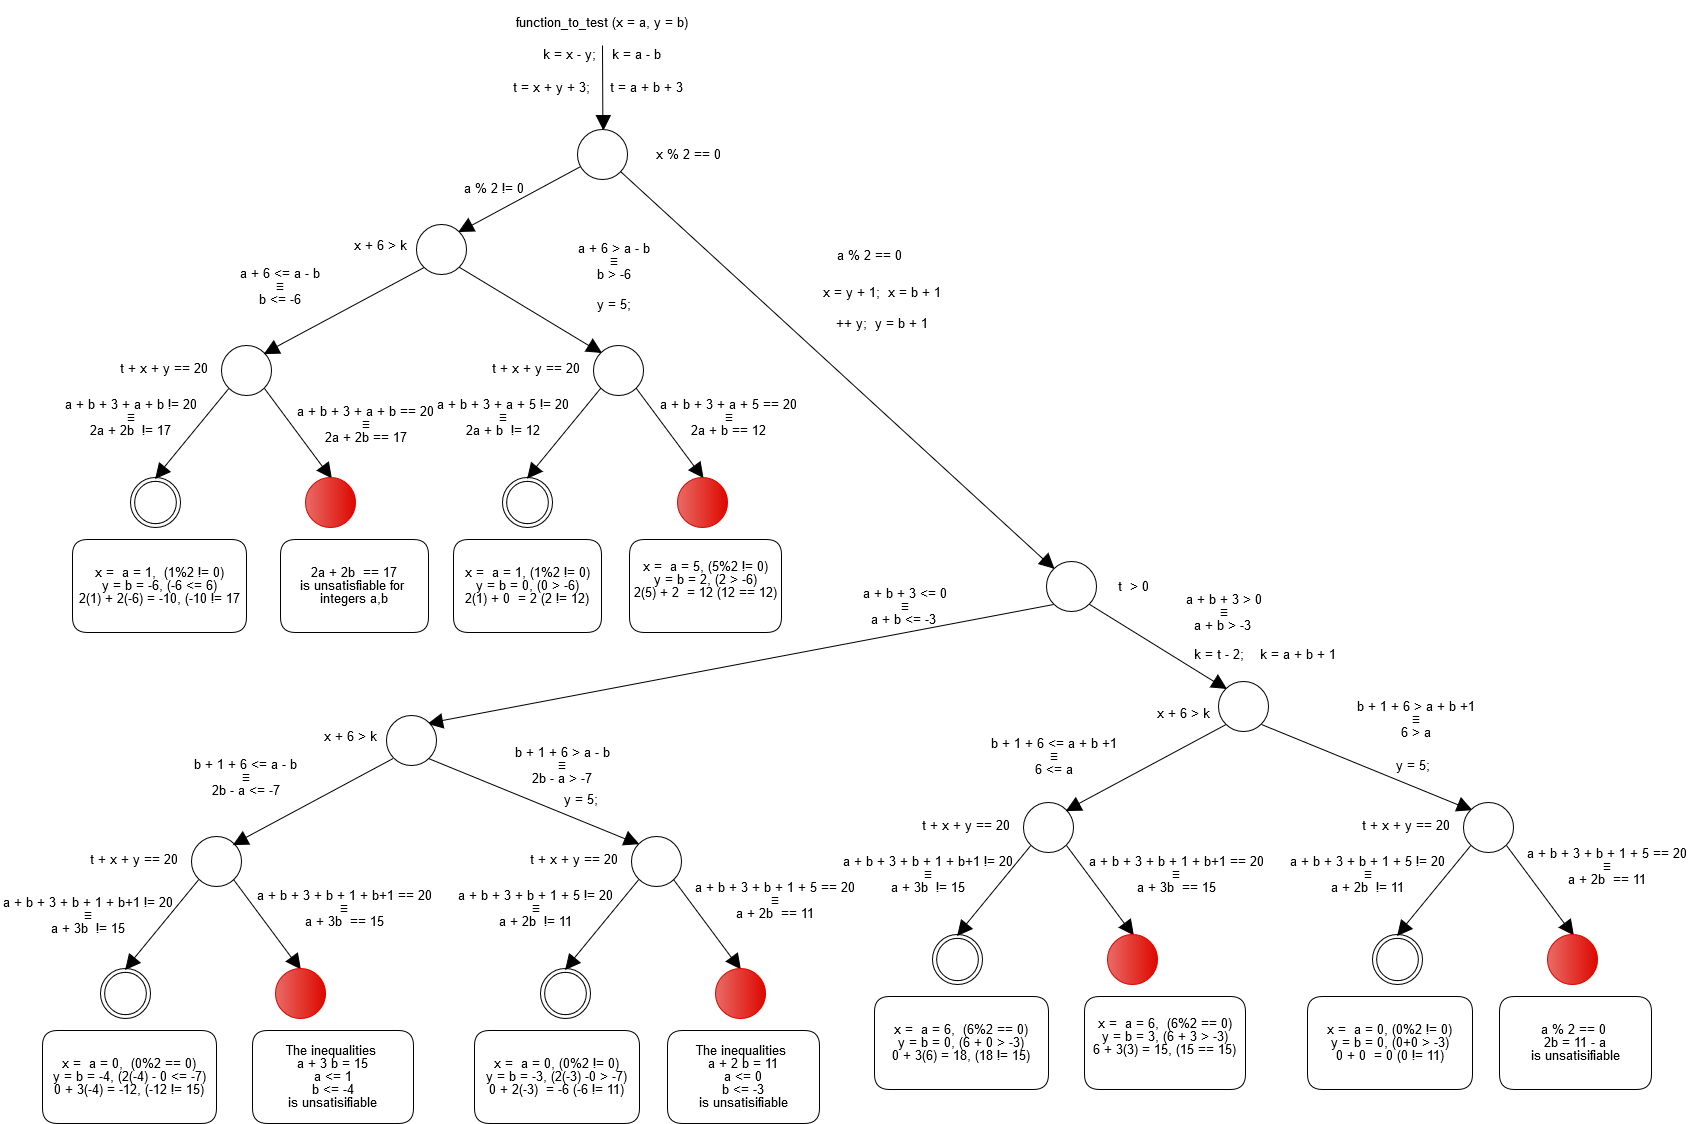
\includegraphics[scale=.30,keepaspectratio=true]{./paths.png}
\end{figure}
\color{black}

\item Please show all the path constraints resulting due to the symbolic execution on the following program.

\color{blue}
The paths are shown in the figure above:

\begin{enumerate}
\item $(a\%2 \neq 0) \wedge (b \leq -6) \wedge (2a + 2b \neq 17)$
\item $(a\%2 \neq 0) \wedge (b \leq -6) \wedge (2a + 2b = 17)$
\item $(a\%2 \neq 0) \wedge (b > -6) \wedge (2a + b \neq 12)$
\item $(a\%2 \neq 0) \wedge (b > -6) \wedge (2a + b = 12)$

\item $(a\%2 = 0) \wedge (a + b \leq -3) \wedge (2b - a \leq -7) \wedge (a + 3b \neq 15)$
\item $(a\%2 = 0) \wedge (a + b \leq -3) \wedge (2b - a \leq -7) \wedge (a + 3b = 15)$
\item $(a\%2 = 0) \wedge (a + b \leq -3) \wedge (2b - a > -7) \wedge (a + 2b \neq 11)$
\item $(a\%2 = 0) \wedge (a + b \leq -3) \wedge (2b - a > -7) \wedge (a + 2b = 11)$

\item $(a\%2 = 0) \wedge (a + b > -3) \wedge (6 \leq a) \wedge (a + 3b \neq 15)$ \label{example}
\item $(a\%2 = 0) \wedge (a + b > -3) \wedge (6 \leq a) \wedge (a + 3b = 15)$
\item $(a\%2 = 0) \wedge (a + b > -3) \wedge (6 > a) \wedge (a + 2b \neq 11)$
\item $(a\%2 = 0) \wedge (a + b > -3) \wedge (6 > a) \wedge (a + 2b = 11)$

\end{enumerate}

\color{black}

\item Additionally, assume that you would like the symbolic execution to identify whether the function has any ``divide by zero" exceptions. How would you modify the symbolic execution to identify such cases?


\color{blue}
Only line 20 uses integer division, therefore we need to ensure the denominator $x$ in $(t+x+y)/x$  to be non zero. To achieve that we can imagine we have an assertion $assert (x \; != 0) $ before line 21. Assuming the path constraint until line 21 is $C$ and the symbolic value of $x$ is $x'$, then if the formula $C \wedge (x' == 0)$ is sat, then there is a ``divide by zero" exception. If the formula is unsat, then this exception wouldn't be thrown. 


Paths that already proved to be unsat or fail some assertions could be excluded.


\color{black}

\item Provide the modified path constraints due to the additional divide by zero checking.

\color{blue}
The following picture shows the paths with division by zero. Note that paths already proved to be unsat or fail the assertion in line 18 are excluded because the execution would not reach line 21.  As shown in the figure, the inputs $x=-2, y = -1$, $x = 6, y = -1$, or $x=0, y = -1$ throw ``divide by zero exception".

\color{blue}
\begin{figure}[H]
 \centering
 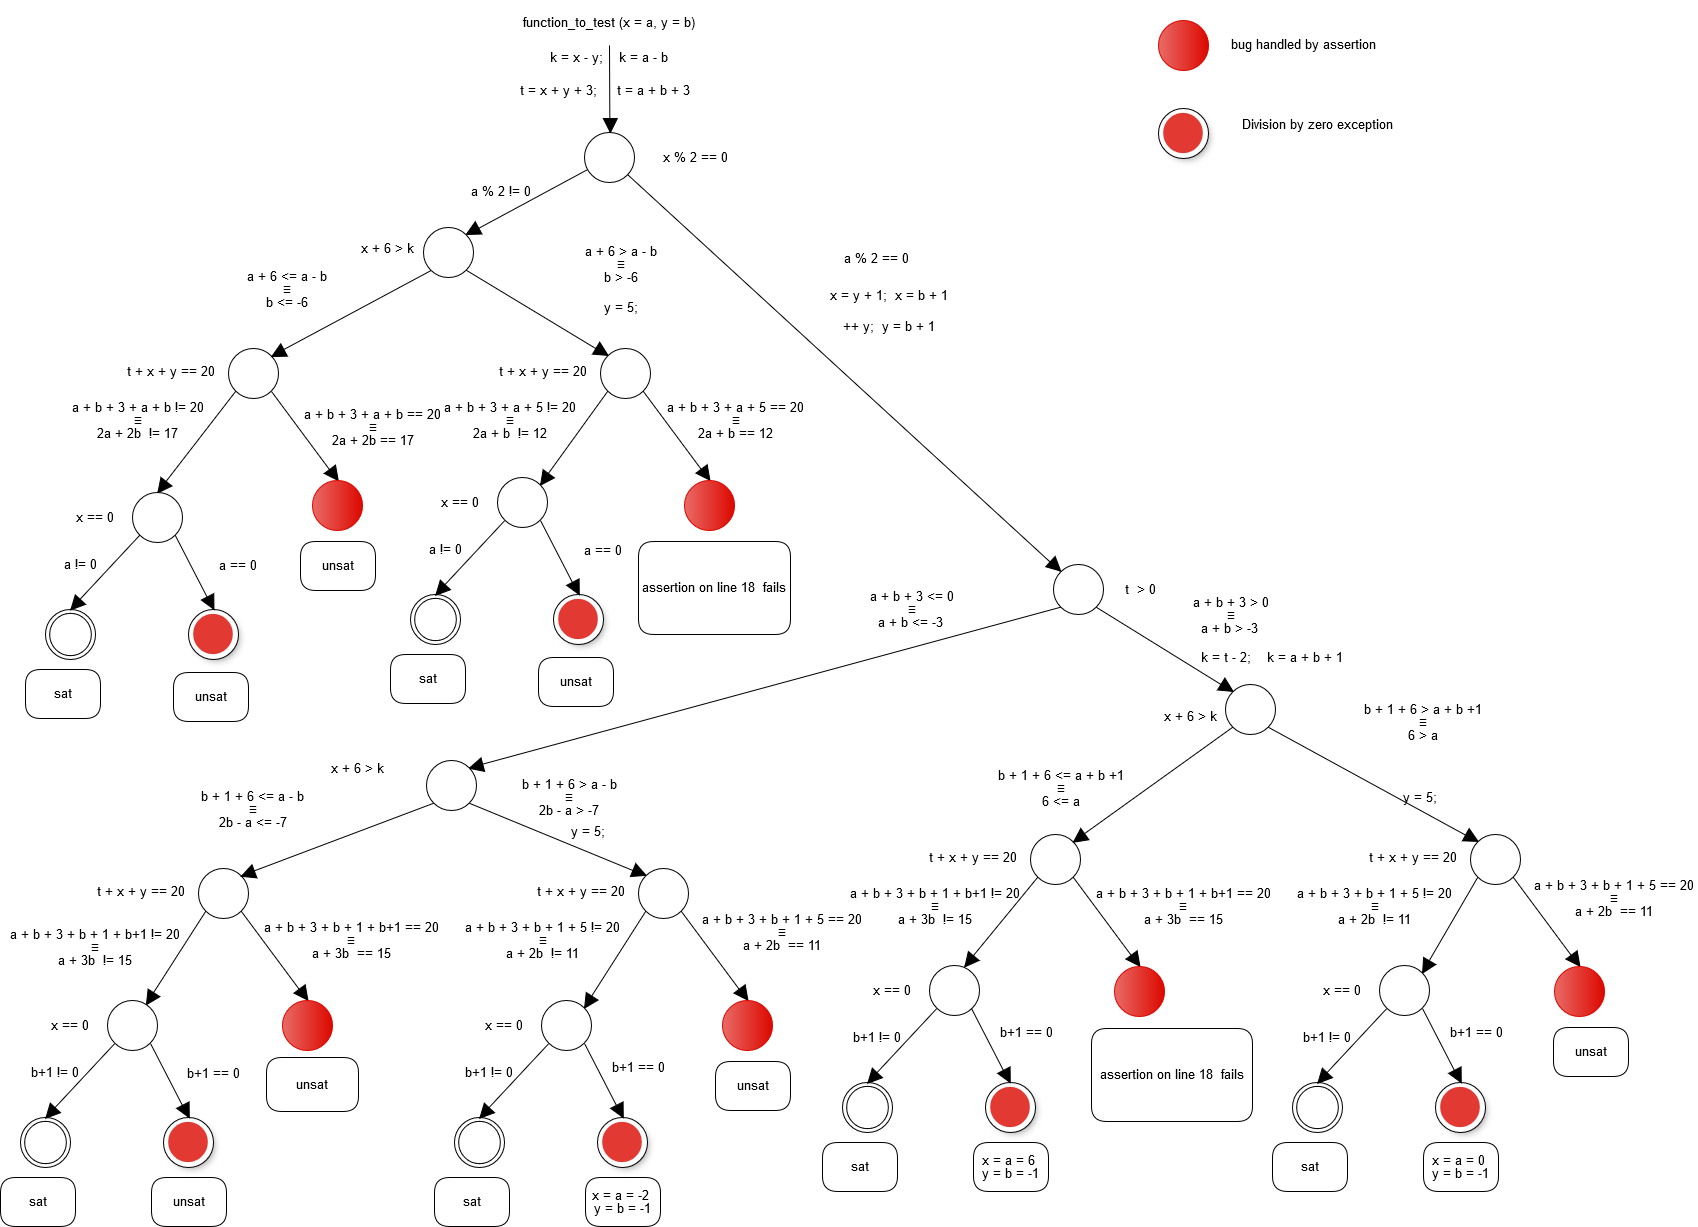
\includegraphics[scale=.30,keepaspectratio=true]{./zero.png}
\end{figure}

Below are the constraints that checks when $x = 0$: 

\begin{enumerate}
\item $(a\%2 \neq 0) \wedge (b \leq -6) \wedge (2a + 2b \neq 17) \wedge (a = 0)$ 
\item $(a\%2 \neq 0) \wedge (b > -6) \wedge (2a + b \neq 12) \wedge (a = 0)$
\item $(a\%2 = 0) \wedge (a + b \leq -3) \wedge (2b - a \leq -7) \wedge (a + 3b \neq 15) \wedge (b + 1 = 0)$
\item $(a\%2 = 0) \wedge (a + b \leq -3) \wedge (2b - a > -7) \wedge (a + 2b \neq 11)\wedge (b + 1 = 0)$
\item $(a\%2 = 0) \wedge (a + b > -3) \wedge (6 \leq a) \wedge (a + 3b \neq 15) \wedge (b + 1 = 0)$
\item $(a\%2 = 0) \wedge (a + b > -3) \wedge (6 > a) \wedge (a + 2b \neq 11) \wedge (b + 1 = 0)$


\end{enumerate}


\color{black}

\item Explain what would change if you were to use concolic execution instead of symbolic execution
while answering sub-question (a) described above.

\color{blue}
Concolic execution assigns random values to the input variables $x$ and $y$. Initially concolic execution starts with an empty path. Then based on the concrete random inputs, the execution traverses the code, and whenever it encounters a branch, it adds the corresponding condition to the path as a conjunction. When it finishes, the path obtained is the path of the random input. To explore other paths, the last condition in the path can be negated and the path formula can be passed to the SMT solver to get an input for that path. 
To explore parent branches, the last condition can be removed and the process can be repeated by negating the last condition in the parent path constraint. 

For example, if the random input is $x = 6, y = 0$, then the concolic execution would get the following constraint:
\begin{align*}
(a\%2 = 0) \wedge (a + b > -3) \wedge (6 \leq a) \wedge (a + 3b \neq 15)
\end{align*}

Negating the last condition would generate this formula
\begin{align*}
(a\%2 = 0) \wedge (a + b > -3) \wedge (6 \leq a) \wedge (a + 3b = 15)
\end{align*}

The SMT solver would return the input $x = 6, y = 3$ which hits the bug. 

\color{black}

\end{enumerate}
\end{enumerate}

\end{document}
